% Generated by tools/export_latex.go. Do not edit.
% Per-image phase breakdown of one evaluation pass (pgfplots); Tier 3 is bounded below by the probe window
% Source: empirical_study.json sha256 1a5f6242aa47c2345354bbe6ba82c883cacd64889d0cff7a6ef100f506bdd97d
% Images are chosen at evenly spaced ranks of total duration.
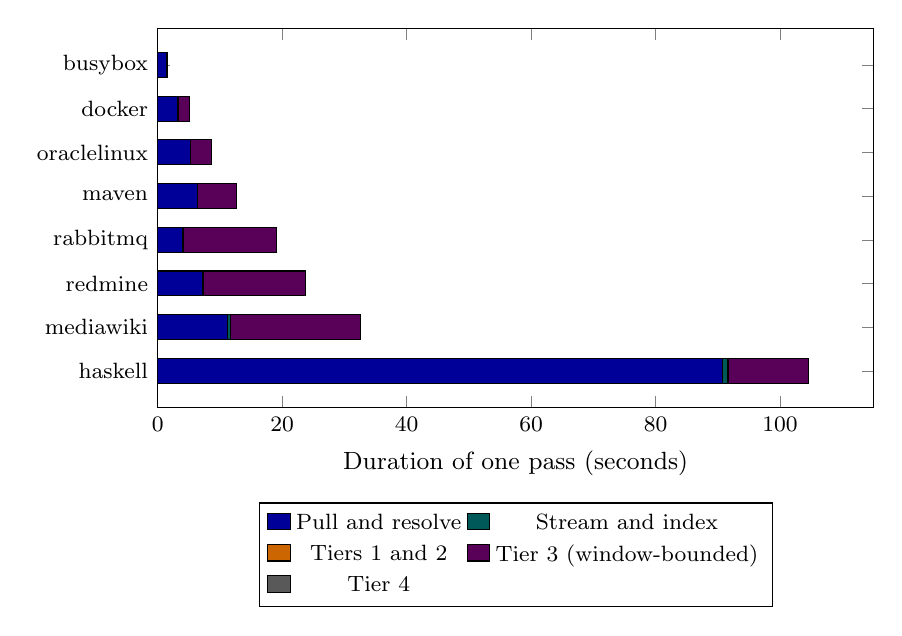
\begin{tikzpicture}
\begin{axis}[
    xbar stacked,
    width=0.88\columnwidth,
    height=6.4cm,
    xlabel={Duration of one pass (seconds)},
    symbolic y coords={busybox,docker,oraclelinux,maven,rabbitmq,redmine,mediawiki,haskell},
    ytick=data,
    xmin=0,
    enlarge y limits=0.12,
    bar width=9pt,
    y dir=reverse,
    legend style={at={(0.5,-0.25)}, anchor=north, legend columns=2, font=\footnotesize},
    tick label style={font=\footnotesize},
    label style={font=\small},
]
\addplot[fill=blue!60!black] coordinates {
    (1.331,busybox)
    (3.232,docker)
    (5.213,oraclelinux)
    (6.362,maven)
    (4.003,rabbitmq)
    (7.118,redmine)
    (11.189,mediawiki)
    (90.732,haskell)
};
\addlegendentry{Pull and resolve}
\addplot[fill=teal!70!black] coordinates {
    (0.001,busybox)
    (0.035,docker)
    (0.099,oraclelinux)
    (0.079,maven)
    (0.054,rabbitmq)
    (0.196,redmine)
    (0.491,mediawiki)
    (0.882,haskell)
};
\addlegendentry{Stream and index}
\addplot[fill=orange!80!black] coordinates {
    (0.000,busybox)
    (0.000,docker)
    (0.004,oraclelinux)
    (0.001,maven)
    (0.002,rabbitmq)
    (0.014,redmine)
    (0.027,mediawiki)
    (0.017,haskell)
};
\addlegendentry{Tiers 1 and 2}
\addplot[fill=violet!70!black] coordinates {
    (0.255,busybox)
    (1.810,docker)
    (3.338,oraclelinux)
    (6.266,maven)
    (15.013,rabbitmq)
    (16.346,redmine)
    (20.880,mediawiki)
    (12.921,haskell)
};
\addlegendentry{Tier 3 (window-bounded)}
\addplot[fill=gray!70!black] coordinates {
    (0.000,busybox)
    (0.000,docker)
    (0.000,oraclelinux)
    (0.000,maven)
    (0.000,rabbitmq)
    (0.000,redmine)
    (0.000,mediawiki)
    (0.000,haskell)
};
\addlegendentry{Tier 4}
\end{axis}
\end{tikzpicture}
